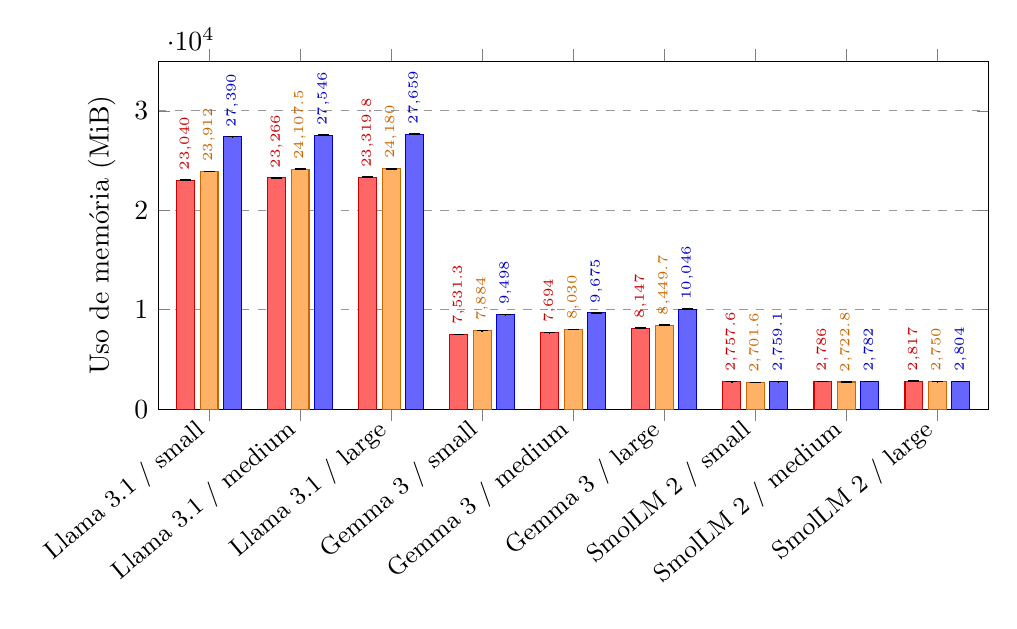
\begin{tikzpicture}
    \begin{axis}[
        % Plot type
        ybar,
        % Plot dimensions
        width            = \textwidth,
        height           = 6cm,
        enlarge x limits = 0.07,
        bar width        = 1.5ex,
        % Labels
        ylabel            = {Uso de memória (MiB)},
        symbolic x coords = {
            {Llama 3.1 / small},
            {Llama 3.1 / medium},
            {Llama 3.1 / large},
            {Gemma 3 / small},
            {Gemma 3 / medium},
            {Gemma 3 / large},
            {SmolLM 2 / small},
            {SmolLM 2 / medium},
            {SmolLM 2 / large}
        },
        x tick label style = {rotate = 40, anchor = east, font = \small},
        % Axes
        ymin = 0,
        ymax = 35000,
        % Labels
        nodes near coords,
        nodes near coords style={
            font   = \tiny,
            rotate = 90,
            anchor = west,
            /pgf/number format/fixed,
            /pgf/number format/precision = 1
        },
        % Grid
        ymajorgrids = true,
        grid style  = {dashed, gray!80}
    ]

        % Q3_K_M
        \addplot+[
            % Bar and label color
            fill                                = red!60,
            draw                                = red!80!black,
            every node near coord/.append style = {color = red!80!black},
            % Error bars
            error bars/.cd,
            y dir = both,
            y explicit,
            error bar style = {black, line width = 0.5pt},
        ] coordinates {
            ({Llama 3.1 / small},  23040.0) +- (0,  5.00)
            ({Llama 3.1 / medium}, 23266.0) +- (0, 37.33)
            ({Llama 3.1 / large},  23319.8) +- (0, 40.18)
            ({Gemma 3 / small},     7531.3) +- (0, 11.44)
            ({Gemma 3 / medium},    7694.0) +- (0,  7.81)
            ({Gemma 3 / large},     8147.0) +- (0, 58.37)
            ({SmolLM 2 / small},    2757.6) +- (0,  4.16)
            ({SmolLM 2 / medium},   2786.0) +- (0,  5.01)
            ({SmolLM 2 / large},    2817.0) +- (0,  6.44)
        };

        % Q4_K_M
        \addplot+[
            % Bar and label color
            fill                                = orange!60,
            draw                                = orange!80!black,
            every node near coord/.append style = {color = orange!80!black},
            % Error bars
            error bars/.cd,
            y dir = both,
            y explicit,
            error bar style = {black, line width = 0.5pt},
        ] coordinates {
            ({Llama 3.1 / small},  23912.0) +- (0,  2.47)
            ({Llama 3.1 / medium}, 24107.5) +- (0, 42.32)
            ({Llama 3.1 / large},  24180.0) +- (0, 32.22)
            ({Gemma 3 / small},     7884.0) +- (0,  9.11)
            ({Gemma 3 / medium},    8030.0) +- (0, 11.04)
            ({Gemma 3 / large},     8449.7) +- (0, 53.86)
            ({SmolLM 2 / small},    2701.6) +- (0,  6.88)
            ({SmolLM 2 / medium},   2722.8) +- (0,  3.69)
            ({SmolLM 2 / large},    2750.0) +- (0,  8.89)
        };

        % Q8_0
        \addplot+[
            % Bar and label color
            fill                                = blue!60,
            draw                                = blue!80!black,
            every node near coord/.append style = {color = blue!80!black},
            % Error bars
            error bars/.cd,
            y dir = both,
            y explicit,
            error bar style = {black, line width=0.5pt},
        ] coordinates {
            ({Llama 3.1 / small},  27390.0) +- (0,  3.05)
            ({Llama 3.1 / medium}, 27546.0) +- (0, 41.65)
            ({Llama 3.1 / large},  27659.0) +- (0, 31.92)
            ({Gemma 3 / small},     9498.0) +- (0,  7.81)
            ({Gemma 3 / medium},    9675.0) +- (0,  9.17)
            ({Gemma 3 / large},    10046.0) +- (0, 51.93)
            ({SmolLM 2 / small},    2759.1) +- (0, 14.13)
            ({SmolLM 2 / medium},   2782.0) +- (0,  2.23)
            ({SmolLM 2 / large},    2804.0) +- (0,  5.00)
        };
    \end{axis}
\end{tikzpicture}
